\chapter{Large-Scale Speech Recognition}
\label{chapter:largescale}

\section{Overview}
End to end speech recognition models have millions of parameters and the architecture complexities make them highly data hungry \cite{Li2020OnRecognition}. Modern \acrshort{asr} systems have been designed to work in multiple domain and environment conditions, and this robustness is possible due to the usage of larger and larger datasets. One of the largest datasets is the 300,000 hours dataset from Google's research team. In their work, they have attempted to build a domain invariant speech recognition model using the large dataset\cite{Narayanan2019TowardTraining}. Other applications include multi-lingual \acrshort{asr} models \cite{Kannan2019Large-ScaleModel} and highly accurate domain-specific \acrshort{asr} models. These experiments showcase the ability of the \acrshort{asr} systems to perform at high levels by using more and more data. An observation from almost all of these works is that the researches are limited to an industrial domain and published by Google, Microsoft, etc who go through fewer budget constraints than other researchers in the domain of \acrshort{asr}. In the academic domain, the amount of research done in this direction is limited due to the resource constrains concerning \acrshort{gpu} resource, CPU resources, network communication availability of datasets, disk storage. 

\section{Scaling up training}
One of the major factors that have led to the rise in popularity of \acrshort{dnn}s, is due to the increase in the scale of data used to train them. There are three main dimensions in which this can be done. First is the magnitude of training data. The model performance can be improved by feeding more data to the deep neural network during training \cite{Hestness2017DEEPEMPIRICALLY}. The definition of a \emph{large-scale} dataset specific to speech recognition is ever-changing. For some context, a popular research in 2014 \cite{Hannun2014DeepRecognition}, used 5000 hours of training data and more recent research in 2020 \cite{Narayanan2019RECOGNIZINGMODELS}, researchers have used 300,000 hours of training data with random augmentation techniques for each epoch. Hence, we can observe that, In the previous 7 years, the training data used in researches has grown by multiple folds. Increasing the amount of high-quality training data hence is one of the unequivocal ways to improve performance of deep learning models. Hence, the practice of adding more and more training data is likely to continue through the next few years \cite{Mayer2020ScalableInfrastructures}. 


The second dimension is the scale of the infrastructure. The easily available parallel hardware, especially graphics processing units (\acrshort{gpu}s), has proven to be a great enabler to train \acrshort{dnn}s in shorter times than before \cite{Zhang2017Poseidon:Clusters}. This is also due to the reducing costs of hardware resources. Storing and handling data have become cheaper and easier \cite{Sayed2014ASecurity}. \acrshort{gpu} resources have become cheaper and more powerful, which have enabled researchers to use more data for training of deep neural networks \cite{Sayed2014ASecurity}. 

The third dimension is the size of the \acrshort{dnn} models, by increasing the width and depth of the models, \acrshort{dnn} models have increased in architectural complexity to achieve better results \cite{Dean2012LargeNetworks}. 

\section{Distributed Training}
Complex models trained on large datasets have shown good results \cite{Dean2012LargeNetworks}. Such huge training tasks can take models a few weeks or even months on a single \acrshort{gpu} to reach convergence. To increase the throughput of the training system, one of the straightforward  methods is by increasing the amount of compute resources, which include the number of \acrshort{gpu}s available. Distributed training is the method of training in a distributed infrastructure of multiple compute nodes, each with multiple \acrshort{gpu}s on it \cite{Langer2020DistributedPerspective}. 

This also brings with it many challenges. The first challenge is to use the computing resources efficiently. This should also go along with tight integration of hardware elements to improve the overall throughput of the system. Data transmissions across machines can be a common bottleneck when training a network. During training a deep neural network using SGD, the weights have to be synchronized across all the devices in use. As the amount of \acrshort{gpu}s in the system grows, the data transmission overhead also grows with it. These challenges require research at a confluence of both computing systems and deep learning training methods, and is receiving growing attention \cite{Xiao2018Gandiva:Learning, Mai2020KungFu:Adaptive, Chilimbi2014ProjectSystem, Cui2016GeePS:Server, Peng2018Optimus:Clusters}.

\subsection{Types of parallelism}
There are many ways to train deep learning models in parallel. The most common ones are discussed here, namely data and model parallelism.

\subsubsection{Model Parallelism}
In model parallelism, split the deep neural network into different devices and load a portion of the model on each device for training, as shown in Figure \ref{fig:modelparallel}. The device that holds the first layer receives the training data. Next, the data propagates through the rest of the forward pass on the device, and it passes the output to the device that holds the next layer of the DL model. During the backward pass, compute the gradients starting from the device that hold the output layer and then propagate the gradients to the devices backward till the device with the input layer. 

\begin{figure}[ht]
  \begin{center}
    % below the size of the figure has been reduced for example
    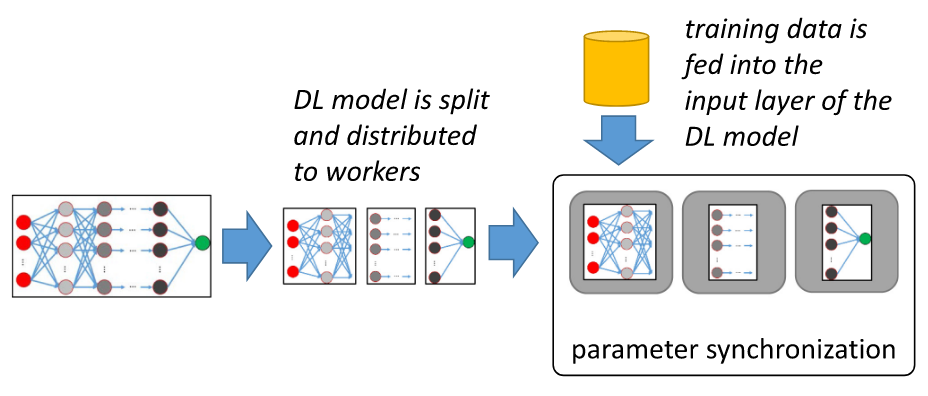
\includegraphics[width=\textwidth]{images/model parallelism.png} 
    \caption{Architecture Diagram of Model Parallelism  \cite{Mayer2020ScalableInfrastructures}}
    \label{fig:modelparallel}
  \end{center}
\end{figure}

The biggest challenge in model parallelism is to split the model into partitions such that the hardware efficiency on different devices is high during training \cite{Mayer2017ThePath}. In many cases, the best way is to empirically try out various permutations and measure the performance and keep the best permutation that has worked well. The second drawback is that model parallelism needs heavy communication between devices. A combined effect of these two challenges is that stalling may occur if models are hard to be split effectively to reduce the communication overloads and synchronization delays. Therefore, training speed might not increase linearly by increasing the number of parallel devices \cite{Mirhoseini2017DeviceLearning}.

The major benefit of the model parallelism is that it can accommodate huge deep learning networks, which cannot be stored on a single device (\acrshort{gpu}) to train them because the memory required to train them is split across multiple units. 

\subsubsection{Data Parallelism}
In data parallelism, copy the deep neural network into different devices and load an identical copy of the model on each device for training, as shown in Figure \ref{fig:dataparallel}. Split the data into the same number as the number of devices, and then data passes into the model replicas of the workers for training. Perform the training process on each chunk of the data that is assigned to the device to generate partial gradient updates of the model parameters. Once it is completed on all the processing units, the parameters are synchronized across all the devices \cite{Koliousis2019CROSSBOW:Servers}. 

\begin{figure}[ht]
  \begin{center}
    % below the size of the figure has been reduced for example
    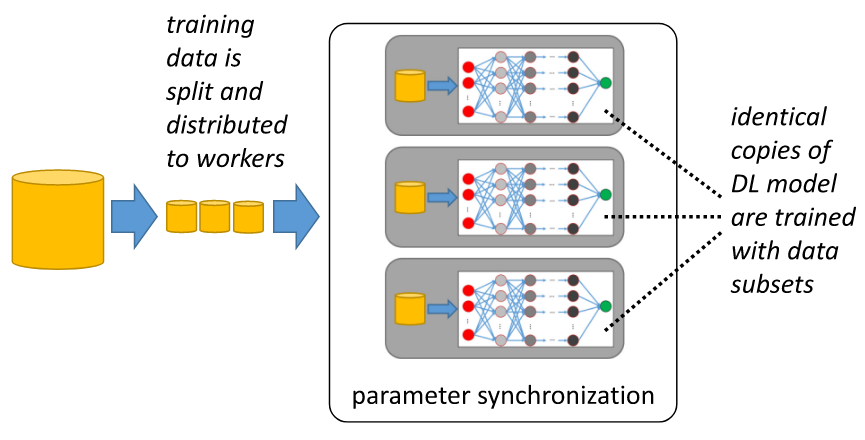
\includegraphics[width=\textwidth]{images/data parallelism.png} 
    \caption{Architecture Diagram of Data Parallelism  \cite{Mayer2020ScalableInfrastructures}}
    \label{fig:dataparallel}
  \end{center}
\end{figure}

Since each device processes a mini batch of data, the total batch size is the product of the mini batch with the number of \acrshort{gpu}s. This high data scale might lead to poor convergence. The other drawback is that ideally, the data that is split along the different workers needs to be identically distributed, so that the parameter updates by the different workers can be easily synchronized to get the overall model \cite{Jia2018BeyondNetworks}.

The major benefit of data parallelism is that it can be easily applied to most of the deep learning networks without much specific knowledge about the architecture of the model. It is highly scalable for the cases when the training is compute intensive but have relatively few parameters like \acrshort{rnn}s, \acrshort{cnn}s \cite{Krizhevsky2014OneNetworks}.


\subsection{Types of synchronization}
Due to the multiple nodes trying to update the model, the important question then becomes when to synchronize the parameters between the parallel workers. The main trade off is between managing training convergence and quality with synchronization cost to update all the models on the parallel workers. There are mainly two methods which are discussed here: synchronous and asynchronous methods.

\subsubsection{Synchronous}
The workers synchronize the weight updates after every batch of data processed. This is implemented in some of the first and prominent methods, like the \acrfull{bsp} \cite{Valiant1990AComputation} method, which is already available in popular data analytics platforms. The main advantage is that the model convergence is easier due to the strict nature of synchronization. However, this method is vulnerable to a situation where \emph{one} single worker stalls the entire training process, especially when the different nodes in the system are heterogeneous in nature \cite{Cipar2013SolvingStaleness}.

Synchronous training is already available in many open-source DL frameworks, such
as TensorFlow \cite{Abadi2016TensorFlow:Systems} and PyTorch \cite{Paszke2019PyTorch:Library}. Most ideally, it is best suited for a system where the nodes involved are homogeneous in nature with similar hardware configurations and hence stragglers are not a significant issue and there are minimal delays from communication.

\subsubsection{Asynchronous}
\label{section:hogwild}
The workers update the model parameters completely independent of other workers. Asynchronous training relies on the theoretical characteristic of SGD that the model convergence is robust to the random ordering of data. The model used by a worker at some point of time might be a stale model because there are no binding guarantees. This makes it difficult to assess model convergence using asynchronous training. However, the advantage is that the workers enjoy great levels of flexibility during training, hence avoiding the straggler problem that is faced in the synchronous method.

\emph{Hogwild} \cite{Niu2011HOGWILD:Descent} is one implementation of the asynchronous training of parallel SGD. Hogwild works by providing all the workers access to a shared memory space, which consists of the model parameters. This is completely lock-free, and hence seems dangerous because new model parameters from one worker can be completely overwritten by another worker without being used at all. Nevertheless, it has been shown that that since model updates are anyway sparse in nature when done sequentially, Hogwild also can achieve results similar to sequential training. This has been applied to large neural networks with good results \cite{Deyringer2017ParallelizationHogwild}. 


\subsection{Data Parallel Systems Architecture}
The architecture of the system defines \emph{how} the parameter synchronization among different workers happens in a data parallel system. There are three major considerations for the system architecture. Firstly, the architecture must be able to scale up to many parallel workers to update the DL model and also read the updated DL model. Secondly, the system needs to be configurable, that is, to be able to manage different parameter settings, etc. The third aspect is to be compatible with widely available inter process communication primitives.

\begin{figure}[ht]
  \begin{center}
    % below the size of the figure has been reduced for example
    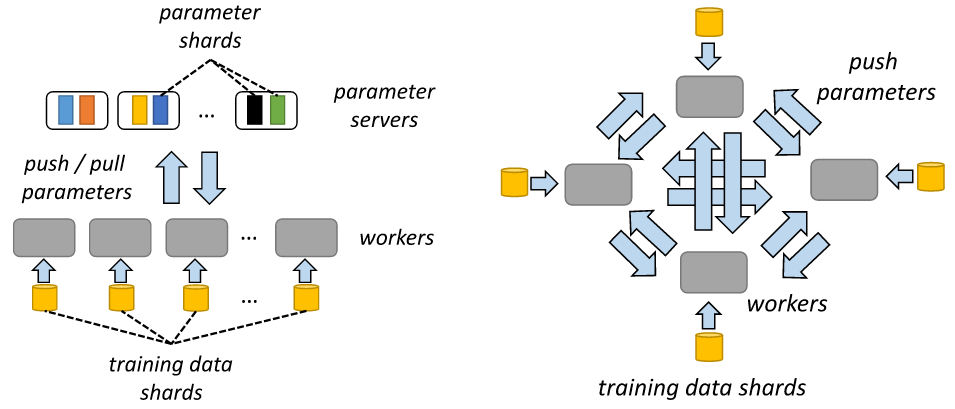
\includegraphics[width=\textwidth]{images/architecture_.png} 
    \caption{Diagram of centralized architecture on the left and decentralized architecture on the right.  \cite{Mayer2020ScalableInfrastructures}}
    \label{fig:arch}
  \end{center}
\end{figure}


\subsubsection{Centralized: Parameter Server}
Centralized architecture consists of a parameter server which is located (logically) in the centre and the worker nodes updates their computed gradients to the central server and all the workers then read the updated model to update their replicas of the model. This architecture is one of the most commonly used in a data parallel system. It is also common to use parameter shards to accelerate the process of communicating the parameter updates. Figure \ref{fig:arch} shows this architecture.

\subsubsection{Decentralized: allreduce Operation}
Decentralized architecture operates without a Parameter Server. The parameters synchronize directly by using an \inlinecode{allreduce} operation as shown in Figure \ref{fig:arch}. 

The major benefit of using a decentralized architecture is that there is no need for one node reserved for parameter server. There is also no single point of failure, and this makes it easier to manage fault tolerance. The major drawback of the decentralized architecture is that communication increases exponentially with the increase in number of workers. One way to avoid this is to use partial gradient updates. For each synchronization, every worker sends a partition of the gradients to every other worker. The communication costs now depend on the number of partitions \emph{and} also on the number of workers in the system. 

Both of these architectures, are widely adopted in leading open-source deep learning frameworks, however the decentralized architecture is the most suitable architecture for a system where there is a single node with multiple \acrshort{gpu}s attached because communication on the same node does not consume too much of resources. However, for multinode training, a centralized architecture works better\cite{Mayer2020ScalableInfrastructures}. 

A quick overview of practical considerations for different types of architecture, parallelism, and synchronization strategy can be accessed here \footnote{Distributed training with TensorFlow, TensorFlow Core. \href{https://www.tensorflow.org/guide/distributed\_training}{https://www.tensorflow.org /guide/distributed\_training} }. 

\section{Related works in large-scale ASR systems}
\label{section:largescale_related}
Large-scale speech recognition has had varying definitions even over the past few years. In 2014, authors applied data and model parallelism for training \acrshort{rnn}-based \acrshort{asr} models \cite{Hannun2014DeepRecognition}. They used 5000 hours of labelled data to build a multi-\acrshort{gpu} powered data-driven speech system which produced state-of-the-art results for that period of time. This solution was also quite robust to distortions and designed to work on both clear, conversational speech and also speech in noisy environments. The work also showed that with data parallelism on more than a few \acrshort{gpu}s, scaling up the overall batch size linearly with the number of \acrshort{gpu}s did not help with the model convergence rate.

More recently, research works from large enterprise companies have continued to focus on increasing the scale of training by multiple folds. Jinyu Li, et al. from Microsoft compare popular end to end speech recognition for large-scale \acrshort{asr} \cite{Li2020OnRecognition}. Authors consider an \acrshort{rnn} transducer, an Attention-based encoder decoder, and transformer architectures and train them with 65,000 hours of training data both for streaming mode and non-streaming modes. In their experiments, to maintain a fair comparison, they have fixed the overall number of parameters to a single limit of around 87M. Their results show that transformer models obtained the best \acrlong{wer}s (\acrshort{wer}) outperforming the other models by around 1\% \acrshort{wer}. They also report that pretraining works well even for large-scale tasks, compared to random initialization.

Google has also worked on increasing their scale of data used for their experiments. In 2019, researches have published their work on building a domain invariant speech recognition model, using large amounts of data from multiple domains to train a single model that work across different applications, sampling rates, audio codecs and formats, and  noise conditions \cite{Narayanan2019TowardTraining}. They claim that their model can adapt to an entirely new domain with as little as one tenth of data compared to that required for a model trained from scratch. This helps to develop speech recognition models for practically any environment with less amount of data. Since then, recent Google research has used datasets that are a huge 300,000 hours in size \cite{Narayanan2019RECOGNIZINGMODELS}. The dataset consists of data from voice search, far field use cases, telephone speech, and audio from YouTube videos. This nature of multi-domain data is again useful for inter-domain speech recognition applications. They also compare the impact of increasing data diversity in improving performance of the models. The authors assess how best to use multi domain data when different proportions of data are available from different domains. They try training models using equal probability from different domain and ignore the relative distribution of data among the domains. From their experiments, this usually tended to overfit the domains that had lesser data. Hence, the overall conclusion was to sample the data from all domain with the probability proportional to the total number of utterances in the domain. Overall, they report that using multi domain data and in large scales improved the output performance of the model significantly.

The previously discussed datasets are not available in public domain, and this has been one of the major issues for developing models for large-scale speech recognition jobs in academic backgrounds. Recent efforts \cite{Galvez2021TheUsage, Pratap2020MLS:Research} have been to create such a publicly available dataset that can be used in academic research. The People's Speech dataset \cite{Galvez2021TheUsage} is a free to download dataset with 31400 hours with more data continuously added. The data, collected by scraping the internet for appropriately licensed audio data with transcriptions. The data collected is diverse in nature, with varying sampling rates, background noise and different forms of speech. There are a few problems with this dataset, as the authors state that there is no defined measure if there are duplicates in the dataset because the dataset's creation is by crawling the internet, it is possible that some data appears twice in the dataset. This also means that creating test sets with no overlap with the training set is challenging. 

Multilingual LibriSpeech (MLS) \cite{Pratap2020MLS:Research} dataset is the first attempt to create a large scale multilingual dataset. It has a total of 32,000 hours of English data and 4,500 hours of data from 7 other languages. The dataset is entirely audiobooks, with  transcriptions downloaded from the internet and then aligned with the audio. This dataset can be used for both speech recognition and text to speech applications since the audio is quite clean with minimal to zero background noise. 

Common Voice \cite{Ardila2020CommonCorpus} is a crowd-sourced multilingual dataset that is mainly focused to propel automatic speech recognition tasks. This dataset is easily scalable for any language because community efforts drives both data collection and data validation. At the time of writing this report, the common voice dataset has 12,500 hours of labelled data \footnote{Common Voice. \href{https://commonvoice.mozilla.org/en}{https://commonvoice.mozilla.org/en}}. For many of the languages in the common voice dataset, it is the only publicly available dataset source for speech recognition tasks. Users can record audio by reading out sentences or phrases that are shown to them through common voice's app or website. The text used in common voice comes mainly from Wikipedia articles. For data validation, a maximum of three volunteers listen to an audio clip and the clip is valid as soon as two votes are positive.

\section{Summary}
It is apparent from industry-based research that there are huge improvements and advantages to be gained from increasing the dataset size used for training the models. There is a lot of work done in this direction to scale up the amount of publicly available speech data that can be used for academic research. \emph{Hence, it is time for researchers in academic field to be well-prepared to scale up training by multiple folds in the near future. The aim of this thesis is to act as a guidebook for scaling up training in multiple steps of the training process.} The next chapters discuss the best methods to store data, loading of data, training using multi-\acrshort{gpu}s, training using multiple processes and reporting performance.

